\chapter{Introduction and Background}

The focus on reduction of greenhouse emissions from fossil fuels is today as important as ever. The rapid ongoing modifications of climate conditions are raising concerns and awareness in this regard. Total anthropogenic greenhouse emissions have continued to increase over 1970 to 2010, with larger absolute increase per decade toward the end of this period, with CO\textsubscript{2} emissions from fossil fuel combustion and industrial processes contributing about 78\% of the total. Annual anthropogenic GHG emissions have increased by 10 Gtons equivalent of CO2 between 2000 and 2010, with this increase directly coming from energy supply (47\%), industry (30\%), transport (11\%) and buildings (3\%) sectors \cite{IPCC2014}.

Global warming causes adverse effect and mutations on natural habitats and natural equilibriums of Earth, and is held responsible for increase of atmospheric temperature, acidification of oceans, melting of the permafrost, increased frequency of extreme weather events and others. As a result, many species struggle to adapt to these new environmental conditions and some are facing extinction. Even human related activities are in danger, as the natural habitat become more and more hostile to plants and animals. In the following sections the phenomenon will be explained in more details, and the role of transportation sector will be highlighted.

\section{Global warming and role of transport section emissions} \label{sec:global_warming}

\emph{Global warming} and \emph{Climate change} are terms used for describing the increase in surface and ocean temperature registered in the last century. Due to the accumulation of greenhouse gases, additional energy is stored in the atmosphere and the oceans, causing ice melting and warming of continents and atmosphere. 

\begin{figure}[h]
  \centering
  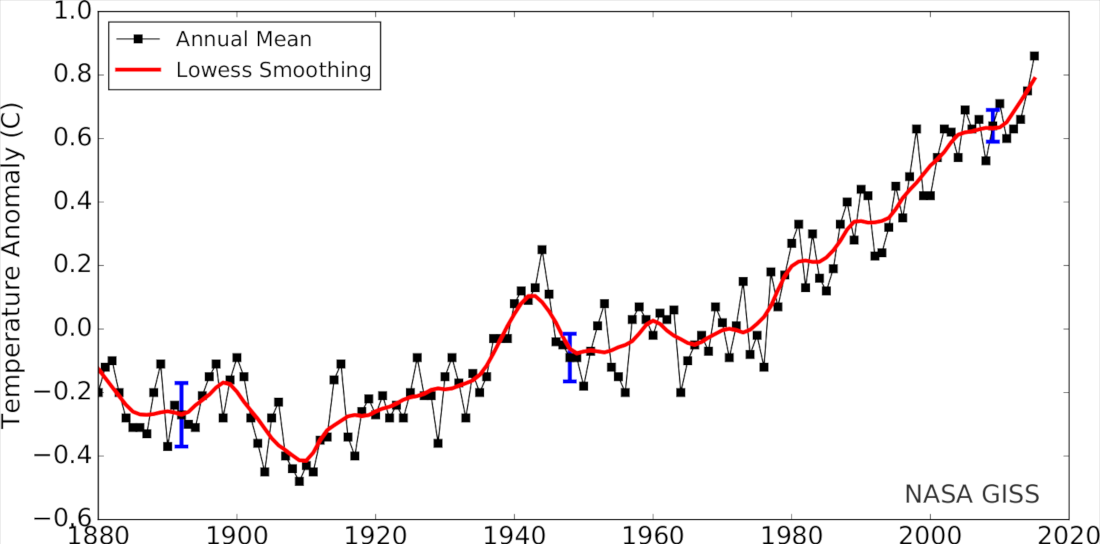
\includegraphics[width=0.8\textwidth]{figures/introduction/temp_rise.pdf}
  \caption{Temperature rise \cite{GISS2016}}
  \label{antropogenic_ghg_emissions}
\end{figure}

Without additional efforts to reduce GHG emissions beyond those in place today, emissions growth is expected to persist driven by growth in global population and economic activities. Baseline scenarios, those without additional mitigation, result in global mean surface temperature increases in 2100 from \SI{3.7}{\celsius} to \SI{4.8}{\celsius} compared to pre-industrial levels \cite{IPCC2014}. Of the 49 Gt CO\textsubscript{2,eq} emitted in 2010, the \emph{transportation} sector is responsible for 14.3\% of the total, ranking as the fourth major emitter economic sector after Electricity and Heat production, Agriculture and Land use, and Industry.

\begin{figure}[h]
  \centering
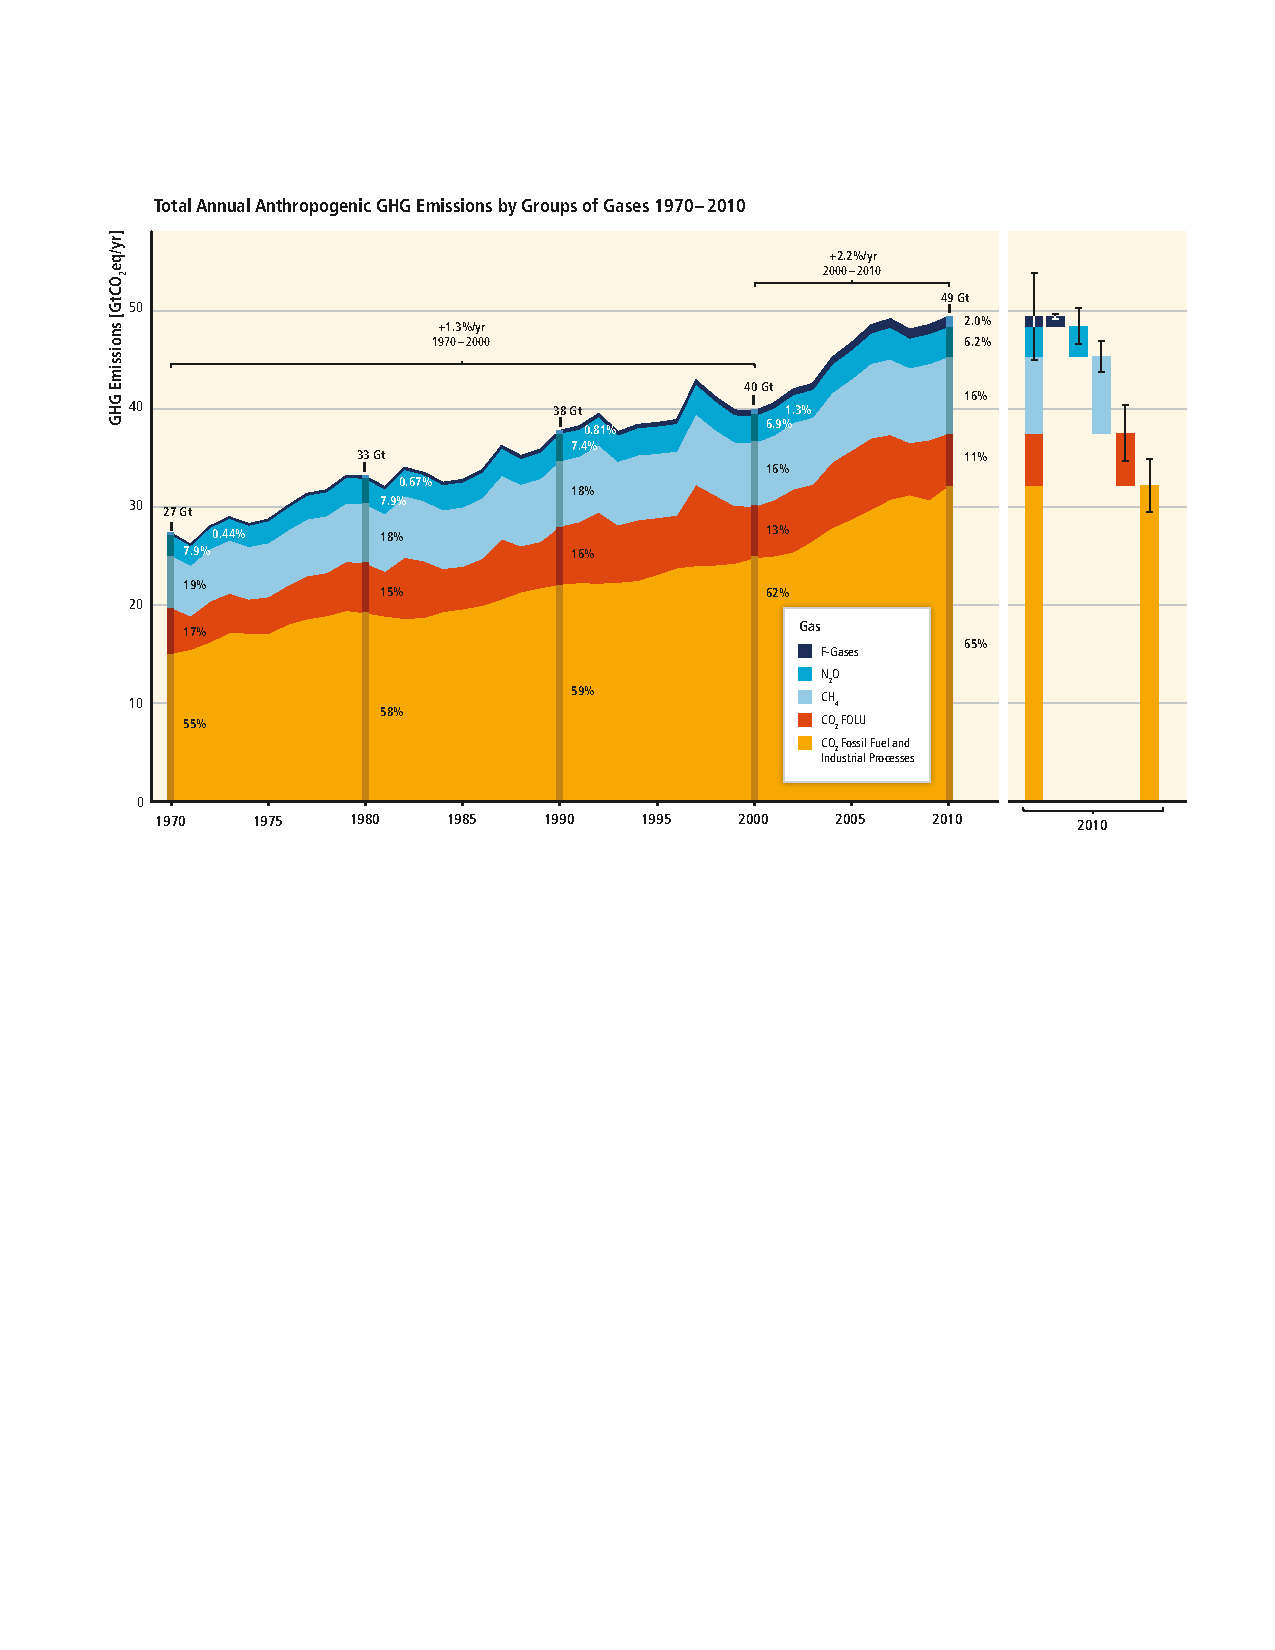
\includegraphics[width=0.8\textwidth]{figures/introduction/antropogenic_ghg_emissions.pdf}
  \caption{Antropogenic GHG emissions by group of gases (1970 - 2010) \cite{IPCC2014}}
  \label{antropogenic_ghg_emissions}
\end{figure}

The scientific community mainly agrees on trying to keep the temperature increase with respect to pre-industrial levels under \SI{2}{\celsius}, equivalent to atmospheric concentrations in 2100 of about 450 ppm CO\textsubscript{2,eq}. The aforementioned scenarios include substantial cuts in anthropogenic GHG emissions by mid century through large scale changes in energy systems and potentially land use. Scenarios reaching these concentrations by 2100 are characterized by lower global GHG emissions in 2050 than in 2010, 40\% to 70\% lower globally, and emissions levels near zero Gt CO\textsubscript{2,eq} or below in 2100 \cite{IPCC2014}. In Figure \ref{fig:mitigationscenarios}, the reduction in emissions for the major economic sectors is reported. It's possible to notice how, especially in the case without heavy implementation of carbon dioxide capture plants, the amount of greenhouse gases released in the atmosphere by transport must be greatly reduced.

\begin{figure}[ht]
  \centering
  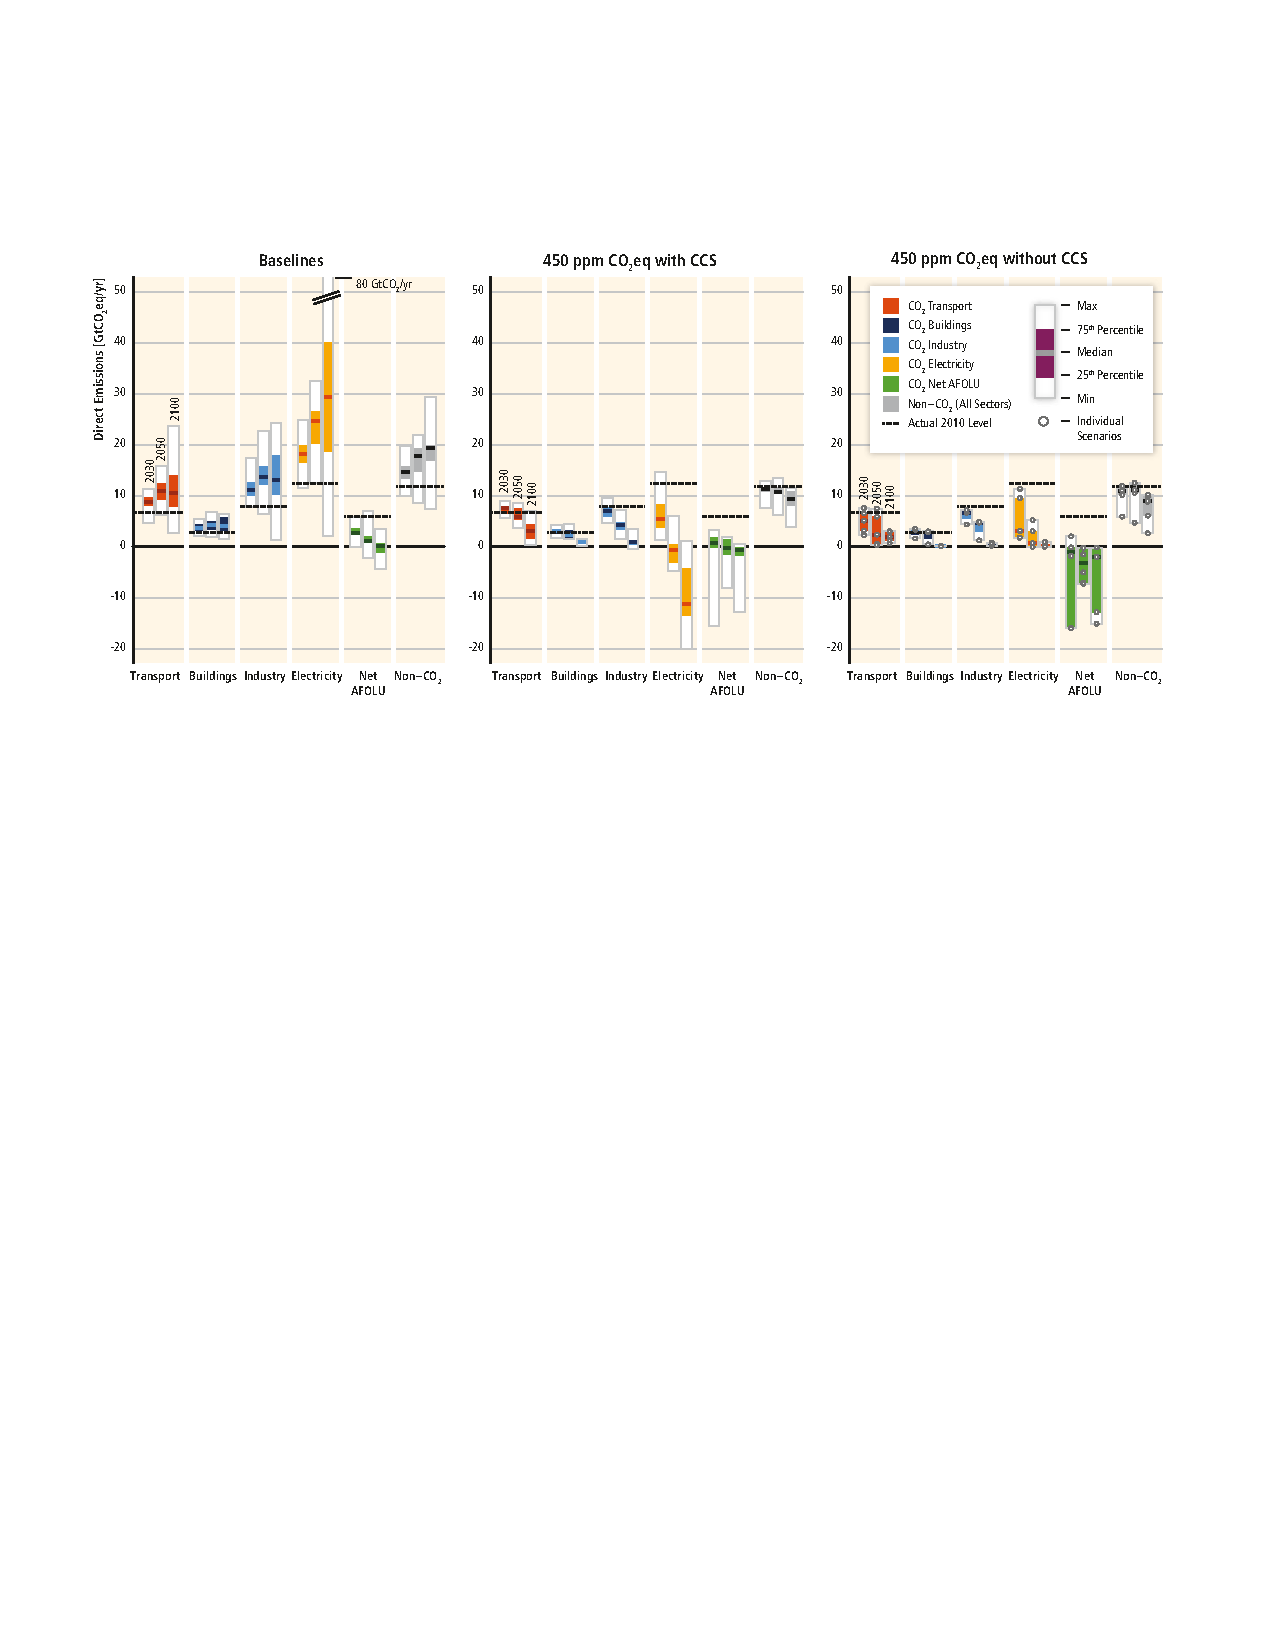
\includegraphics[width=\textwidth]{figures/introduction/mitigation_scenarios.pdf}
  \caption{Review of different mitigation scenarios for 450 ppm \label{fig:mitigationscenarios}}
\end{figure}

The chart represents a review of the major models and scenarios available to date, and taken into consideration in \cite{IPCC2014}. According to the same study, efficiency enhancements and behavioural changes aimed at reducing energy demand compared to baseline scenarios without compromising development, are a key mitigation strategy in scenarios reaching atmospheric CO\textsubscript{2,eq} concentrations of about 450 to about 500 ppm by 2100.

The transport sector accounted for 27\% of final energy use and 6.7 Gt CO\textsubscript{2} direct emissions in 2010, with baseline CO\textsubscript{2} emissions projected to approximately double by 2050. Technical and behavioural mitigation measures for all transport modes, plus new infrastructure and urban redevelopment investments, could reduce final energy demand in 2050 by around 40\% below the baseline \cite{IPCC2014}.

A study by Unger and al.~\cite{Unger2010} attributes a radiative forcing value to different economic sectors that are the main emitters in today economy. The radiative forcing concept has been developed in order to quantify the human and natural influence on the climate system, and is defined as the net energy flux difference at the top of the atmosphere. In Figure~\ref{fig:radiative_forcing}, the positive and negative contributions of the different economic sectors are presented. It's important to notice how on-road transportation is foreseen to be the major responsible for increasing of atmospheric energy content in 2020, and the second most important factor in 2100. This is due to the peculiar composition of exhaust gases produced by vehicles: the production is  mainly constituted by components that contribute to trapping heat. Other sectors, as the power sector, produce much more components that trap heat, but the net contribution is reduced by the amount of components as black-carbon, that reflects the solar radiation and contribute to cooling down the atmosphere. 

\begin{figure}[ht]
  \centering
  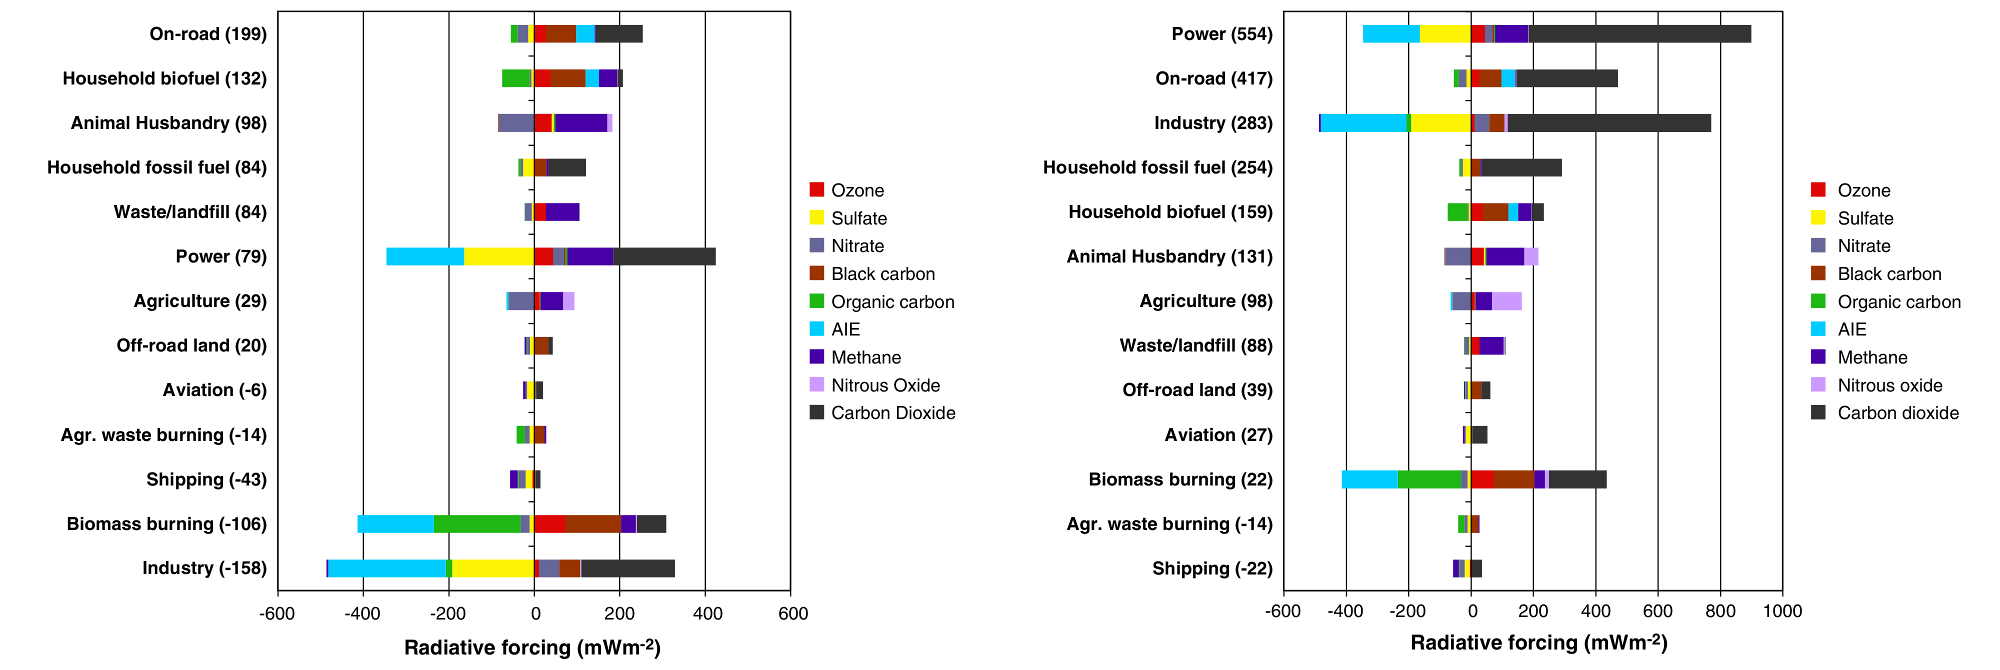
\includegraphics[width=\textwidth]{figures/introduction/radiative_forcing.png}
  \caption{Radiative forcing due to 2000 level emissions grouped by sector in a) 2020 and b) 2100 \label{fig:radiative_forcing}}
\end{figure}

\section{Current transportation scenario}

The average efficiency of modern internal combustion engines is measured to be around 32\% - 36\% for Diesel engines, and around 29\% - 32\% for Gasoline engines.

According to the evidence reported in section~\ref{sec:global_warming}, being the transportation sector one of the main culprits for global warming, an increase in efficiency of passenger vehicles can play an important role in mitigating climate change. Figure~\ref{fig:average_fuel_efficiency} shows how, in the 1980 - 2014 considered timeframe, the specific fuel consumption of U.S. vehicles has been reduced thanks to technical advancements~\cite{BureauofTransportationStatistics2016}.

\begin{figure}[ht]
  \centering
  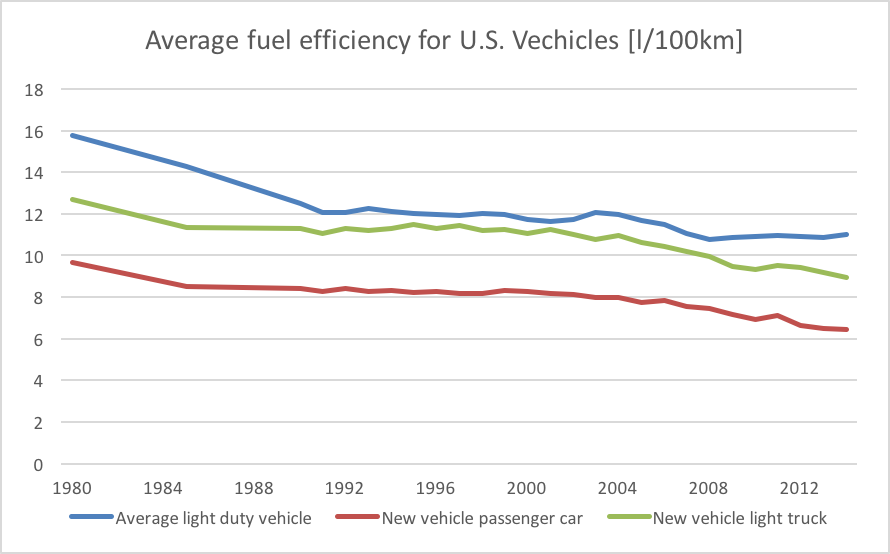
\includegraphics[width=0.8\textwidth]{figures/introduction/average_fuel_efficiency.png}
  \caption{Average fuel efficiency for U.S. vehicles \label{fig:average_fuel_efficiency} }
\end{figure}

Taking a more in depth look at the emissions figure of the transportation economy itself, when considering the energy use by transportation mode in 2013, Highwway is by far the sector that consumes the greater share of the total (83.2\%), followed by Air transportation (6.9\%) and Water transportation (3.9\%). The Highway energy usage can be once again split between Light-duty (52.2\%), Combination Truck (15.3\%), Single-unit truck (7.6\%), and Bus (1.1\%). Certified air carriers experienced the largest total decrease in fuel consumption, consuming about 3.6 billion fewer gallons of jet fuel in 2014 than in 2000. General aviation gasoline showed the largest percent decrease in fuel consumption from 2000 to 2014, declining by 40.8 percent. Additionally, water modes powered by residual fuel oil also showed a large decrease, declining by nearly 2.6 billion gallons during the same period. Consistent with increases in vehicle-miles traveled, light-duty highway vehicles used about 430 million more gallons of gasoline in 2014 than in 2000~\cite{BureauofTransportationStatistics2016a}.

According to the evidence shown, the amount of effort spent on researching and experimenting new and more advanced ways of reducing transportation energy consumption is justified. Numerous different technical trends are nowadays gaining traction in the automotive field, such as downsizing and turbocharging of gasoline engines, or the usage of different cycles. A more in depth analysis will be provided in Section~\ref{sec:technology_improvements}.

\section{Objectives and structure of the thesis}

The main objective of the thesis is to compare three different technologies that aim at recovering waste heat produced by the internal combustion engine. In particular, two different \emph{Organic Rankine} bottoming \emph{Cycles} (ORC) paired with an Otto-cycle engine, and a \emph{Split-Cycle Engine} with \emph{isothermal compression} and \emph{integrated waste heat recovery}.

The comparison will be performed via MATLAB/Simulink simulations. A backward-looking model will take as input the velocity profile of a driving cycle for which experimental data is available, then the torque and angular speed at the engine will be calculated through a simulated transmission. Furthermore, engine maps will be extracted from experimental data along with characteristics and performances of the heat exchangers, making possible the calculation of flow rate, temperature and heat flux for both the exhaust gases and the coolant. Once the waste heat data will be available, the bottoming cycle model will be introduced. Starting from the output of the powertrain model, the recovered energy and produced power will be calculated.

\emph{ADD METHODOLOGIES MODEL SPLIT-CYCLE}

\emph{TO BE CONTINUED WITH STRUCTURE}


%%% Local Variables:
%%% mode: latex
%%% TeX-engine: xetex
%%% TeX-master: "thesis"
%%% End:
%%% \end{document}
